\documentclass[tikz]{standalone}
\usepackage{tikz}
\usepackage{amsmath}
\usepackage{mathrsfs}
\usepackage{amssymb}
\usepackage{amsthm}
\usepackage{booktabs}
\usetikzlibrary{arrows.meta,positioning,calc,backgrounds,shapes,matrix,backgrounds}

\usepackage{xcolor}
% \pagecolor{gray!5}

\tikzset{
  >={Latex},
  flight/.style = {-{Latex}, line width=1.5pt, blue},
  flightGhost/.style = {-{Latex}, line width=1pt, black, dashed},
  timeaxis/.style = {line width=1pt, ->},
  labelNode/.style = {font=\scriptsize, align=center},
  conflict/.style = {red, densely dotted, line width=1pt},
}

\begin{document}
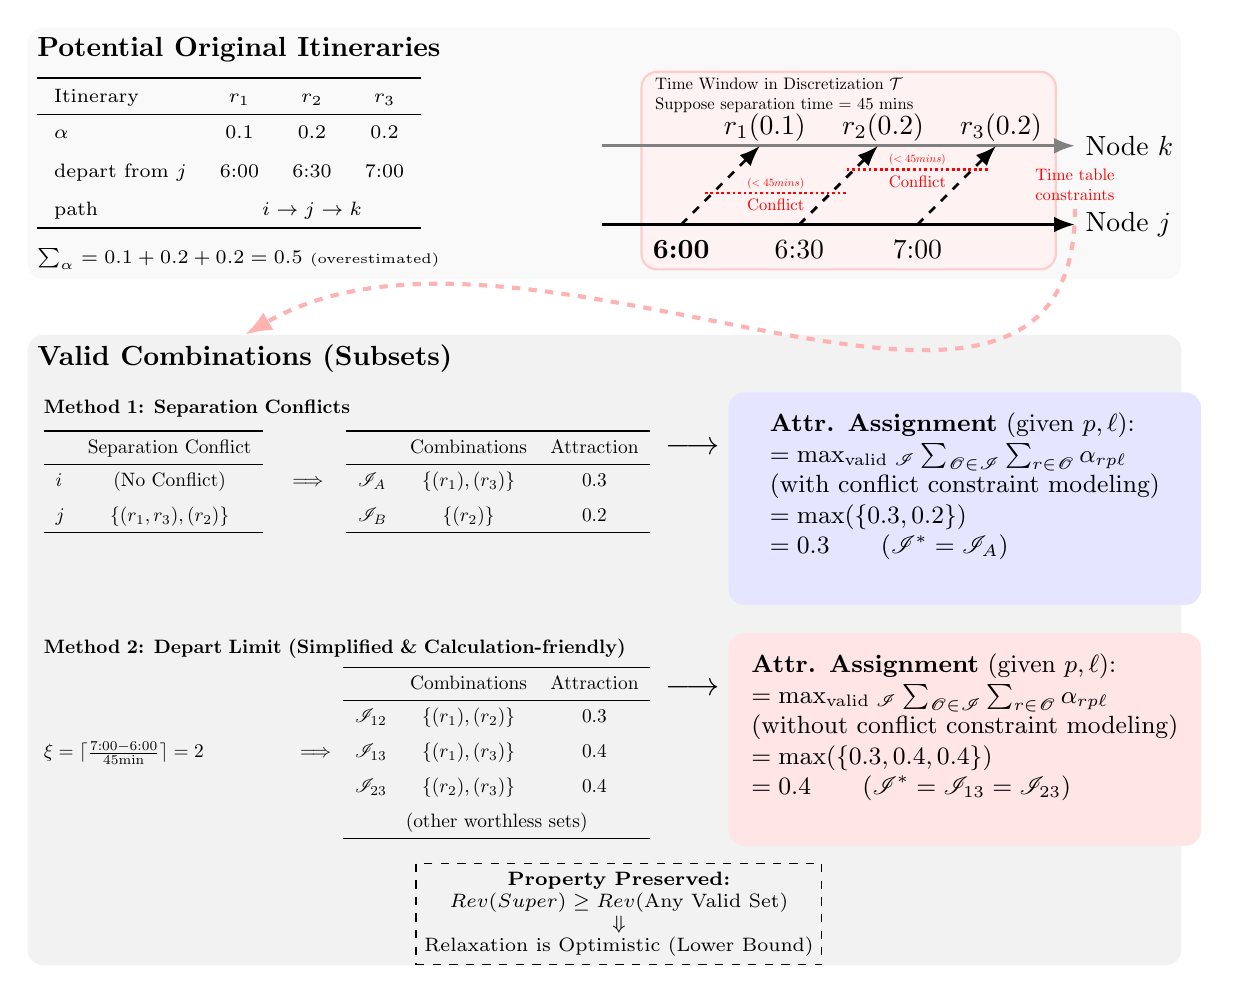
\begin{tikzpicture}
  \def\xScale{1.5}
  \def\yScale{0.8}
  
  % --- Scope 1: Potential Itineraries & Conflicts ---
  \begin{scope}[shift={(-3,0)}, anchor=north west]
    \node[font=\bfseries] (title1) at (0, 2.5) {Potential Original Itineraries};
    \begin{scope}
      % PS: suppose cooldown/separation time is 45 minutes
      \node[labelNode, align=left, anchor=north west] (labelNode) at (0, 2) {
        % Suppose separation time = 45 mins \\
        \begin{tabular}{lccc}
          \toprule
          Itinerary & $r_1$ & $r_2$ & $r_3$ \\
          \midrule
          $\alpha$ & 0.1 & 0.2 & 0.2 \\ [6pt]
          depart from $j$ & 6:00 & 6:30 & 7:00 \\ [6pt]
          path & \multicolumn{3}{c}{$i\to j \to k$} \\
          \bottomrule
        \end{tabular}
        \\ [6pt]
        $\sum_{\alpha} = 0.1+0.2+0.2=0.5$ {\tiny(overestimated)}
      };
    \end{scope}
    \begin{scope}[shift={(7.3,0)}, anchor=north west]
      \draw[timeaxis] (0,0) -- (6,0) node[right, scale=1] (jlabel) {Node $j$};
      \draw[timeaxis, gray] (0,1) -- (6,1) node[right, black, scale=1] (klabel) {Node $k$};
      
      % r1 at t=1
      \draw[flightGhost] (1,0) node[below=2pt] (node_j1) {\textbf{6:00}} -- ++(1,1) node[midway, above, black, align=left, yshift=12pt, xshift=16pt] {$r_1 (0.1)$};
      % r2 at t=2 (too close to r1, separation=1.5)
      \draw[flightGhost] (2.5,0) node[below=2pt] (node_j2) {6:30} -- ++(1,1) node[midway, above, black, align=left, yshift=12pt, xshift=16pt] {$r_2 (0.2)$};
      % r3 at t=3 (compatible with r1, too close to r2)
      \draw[flightGhost] (4,0) node[below=2pt] (node_j3) {7:00} -- ++(1,1) node[midway, above, black, align=left, yshift=12pt, xshift=16pt] {$r_3 (0.2)$};
      
      % Conflict markers
      \draw[conflict] (1.3, 0.4) -- ++(1.8, 0) node[midway, below, red, scale=0.6] {Conflict} ++(0,0.4) node[midway, above, red, scale=0.4] {($<45 mins$)};
      \draw[conflict] (3.1, 0.7) -- ++(1.8, 0) node[midway, below, red, scale=0.6] {Conflict} ++(0,0.4) node[midway, above, red, scale=0.4] {($<45 mins$)};

      % time window
      \path let \p1 = (node_j1.west),
                \p2 = (klabel.north)
      in
        coordinate (timeWindowStart) at (\x1 - 0.3, \y2 + 1);
      \path let \p1 = (node_j3.east),
                \p2 = (node_j3.south)
      in
        coordinate (timeWindowEnd) at (\x1 + 0.3, \y2 - 0.1);
    \end{scope}

    % lower background
    \begin{pgfonlayer}{background}
      \path let \p1 = (jlabel.east),
                \p2 = (labelNode.south)
      in
        coordinate (bgEnd) at (\x1,\y2);
      \fill[gray!5, rounded corners=2mm] (title1.north west) rectangle (bgEnd);
      % rectangle for time window
        \path let \p1 = (timeWindowStart),
                  \p2 = (title1.south east)
        in
          coordinate (timeWindowFrameStart) at (\x1,\y2);
        \draw[thick, red!20, fill=red!5, rounded corners=2mm, on background layer] ($(timeWindowFrameStart)$) rectangle ($(timeWindowEnd)+(1.3,0)$);
        % left up corner label
        \node[scale=0.6, align=left] at ($(timeWindowFrameStart)+(0.1,0)$) {
            Time Window in Discretization $\mathcal{T}$ \\
          Suppose separation time = 45 mins
        };
    \end{pgfonlayer}
  \end{scope}
  
  % --- Scope 2: Valid Combinations ---
  \def\nodeHeight{2.7cm}
  \begin{scope}[shift={(-3,-2.0)}, anchor=south west]
    \node[font=\bfseries] (title2) at (0, 0) {Valid Combinations (Subsets)};

    \matrix[
      anchor=north west,
      ampersand replacement=\@,
      row sep=10pt,
      column sep=0pt
    ] {
      \node[
        align=left,
        anchor=north west,
        scale=0.7,
        transform shape,
        text width=11cm,
        minimum height=\nodeHeight
      ] {
      \textbf{Method 1: Separation Conflicts}\\[6pt]
      \begin{tabular}{lc}
        \toprule
        & Separation Conflict\\
        \midrule
        $i$ & (No Conflict)\\[6pt]
        $j$ & $\{(r_1,r_3), (r_2)\}$\\
        \bottomrule
      \end{tabular}
      \hfill$\implies$\hfill
      \begin{tabular}{lcc}
        \toprule
        & Combinations & Attraction\\
        \midrule
        $\mathscr{I}_A$ & $\{(r_1),(r_3)\}$ & 0.3\\[6pt]
        $\mathscr{I}_B$ & $\{(r_2)\}$ & 0.2\\
        \bottomrule
      \end{tabular}
      };
      \@
      \node[align=left, anchor=north east, minimum height=\nodeHeight] {\large $\longrightarrow$ \\ \\ \\};
      \@
      \node[align=left, font=\small, fill=blue!10, rounded corners=2mm, minimum width=6cm, minimum height=\nodeHeight] {
        \textbf{Attr. Assignment} (given $p,\ell$):\\
        $= \max_{\text{valid } \mathscr{I}} \sum_{\mathscr{O} \in \mathscr{I}} \sum_{r \in \mathscr{O}} \alpha_{rp\ell}$\\
        (with conflict constraint modeling)\\
        $= \max(\{0.3, 0.2\})$\\
        $= 0.3 \qquad(\mathscr{I}^{*}=\mathscr{I}_A)$ \\
      };
      \\
      \node[
        align=left,
        anchor=north west,
        scale=0.7,
        transform shape,
        text width=11cm,
        minimum height=\nodeHeight
      ] {
        \textbf{Method 2: Depart Limit (Simplified \& Calculation-friendly)}\\ [3pt]
        $\xi = \lceil\frac{7:00 - 6:00}{45 \text{min}}\rceil = 2$
        \hfill$\implies$
        \begin{tabular}{lcc}
          \toprule
          & Combinations & Attraction\\
          \midrule
          $\mathscr{I}_{12}$ & $\{(r_1),(r_2)\}$ & 0.3\\[6pt]
          $\mathscr{I}_{13}$ & $\{(r_1),(r_3)\}$ & 0.4\\[6pt]
          $\mathscr{I}_{23}$ & $\{(r_2),(r_3)\}$ & 0.4\\[6pt]
          \multicolumn{3}{c}{(other worthless sets)}\\
          \bottomrule
        \end{tabular}
      };
      \@
      \node[align=left, anchor=north east, minimum height=\nodeHeight] {\large $\longrightarrow$ \\ \\ \\};
      \@
      \node[align=left, font=\small, fill=red!10, rounded corners=2mm, minimum width=6cm, minimum height=\nodeHeight] {
        \textbf{Attr. Assignment} (given $p,\ell$):\\
        $= \max_{\text{valid } \mathscr{I}} \sum_{\mathscr{O} \in \mathscr{I}} \sum_{r \in \mathscr{O}} \alpha_{rp\ell}$\\
        (without conflict constraint modeling)\\
        $= \max(\{0.3, 0.4, 0.4\})$\\
        $= 0.4 \qquad(\mathscr{I}^{*}=\mathscr{I}_{13}=\mathscr{I}_{23})$ \\
      }; \\
    };
  \end{scope}

  \node[below=0.1cm of current bounding box.south, align=center, font=\scriptsize, draw, dashed, inner sep=3pt] (conclusion) {
      \textbf{Property Preserved:}\\
      $Rev(Super) \ge Rev(\text{Any Valid Set})$\\
      $\Downarrow$\\
      Relaxation is Optimistic (Lower Bound)
  };

  \path let \p1 = (bgEnd),
            \p2 = (conclusion.south east)
      in
        coordinate (bgEnd2) at (\x1,\y2);
  \begin{pgfonlayer}{background}
    \fill[gray!10, rounded corners=2mm, on background layer] (title2.north west) rectangle (bgEnd2);
  \end{pgfonlayer}

  % arrow
  \path let \p1 = (jlabel.east), \p3 = (klabel.east),
            \p2 = (jlabel.west)
      in
        coordinate (downArrowStart) at (\x2,{(\y1+\y3)/2});
  \path let \p1 = (title2.north),
            \p2 = (title2.center)
      in
        coordinate (downArrowEnd) at (\x2,\y1);
  \draw[dashed, ->, red!30, line width=1.5pt] ($(downArrowStart) + (0,-0.3)$) to[out=-90, in=30] (downArrowEnd);
  \node[scale=0.6, red, align=center] at ($(downArrowStart)$) {Time table \\ constraints};
  % \node[font=\large, below=0.1cm of downArrowPos] (downArrow) {$\downarrow$};

\end{tikzpicture}
\end{document}
